\mychapter{2}{TWT GmbH Science \& Innovation: Verification of Procedures of Subset
026 chapter 5}
\label{sec:twt}
This sections reports on the modeling of the procedures described in Subset 026 chapter 5---that is, the behavioral part of the ETCS. The goal of the activity is to validate the specification and to support the modeling using SCADE and the verification of SCADE models on a higher level of abstraction in comparison to SCADE models.

The activity is described in the Verification and Validation Plan (see Sect.~6.1.2.5). In short, we provide feedback regarding ambiguities, inconsistencies and errors in the current ETCS standard based on our formalization of the specification using mathematical modeling languages.

\section{Object of verification}

The object of verification is Subset-026 chapter 5 of the specification. We formally model parts of the specification and use the resulting model to validate the specification. This design step has been described in D2.3 (see Sect.~4.4).

\section{Available specification}

The specification is described in Subset-026 chapter 5. It describes procedures of ETCS entities (i.e., required reactions on events and received messages), thereby focusing on required change in status and mode of entities considered.


\section{Detailed verification plan}

\subsection{Goals} 

The goal is to model the the procedures described in Subset-026 chapter 5, thereby focusing on modeling the \textit{system behavior}---that is, the control flow of the on-board unit and the interplay with its environment (e.g., the driver and the RBC). The model is then used to validate the specification.

\subsection{Method/Approach}

As a formal model, we use \textit{colored Petri nets} (CPNs)~\cite{CPN-book}, an extension of classical Petri nets~\cite{PNbook} with data, time, and hierarchy. CPNs are well-established and have been proven successful in numerous industrial projects. They have a formal semantics and with CPN Tools~\cite{Westergaard2013apn}, there exists an open source tool for modeling CPNs. Moreover, CPN Tools also comes with a simulation tool and a model checker, thereby enabling formal analysis of CPN models. 

We focus on modeling the \textit{system behavior}---that is, the control flow of the on-board unit and the interplay with its environment (e.g., the driver and the RBC). Figure~\ref{fig:Top} depicts the CPN representing the highest level of abstraction. It shows the decomposition of the overall system into the on-board unit and its environment: the driver, the RBC, the RIU, the STM, and the GSM module. Each component is modeled as a subpage (i.e., a component). Graphically, a subpage is depicted as a rectangle with a double-lined frame. Furthermore, the model shows through which message channels and shared variables the on-board unit is connected to its environment. A channel or shared variable is modeled by a place which is graphically represented as an elipse. As an example, the driver (i.e., subpage \texttt{Driver}) may send a message to the on-board unit (i.e., subpage \texttt{On-board Unit}) via the place \texttt{msg from driver}, and receives messages sent by the on-board unit via the place \texttt{msg to driver}.

\begin{figure}[tb]
	\centering
		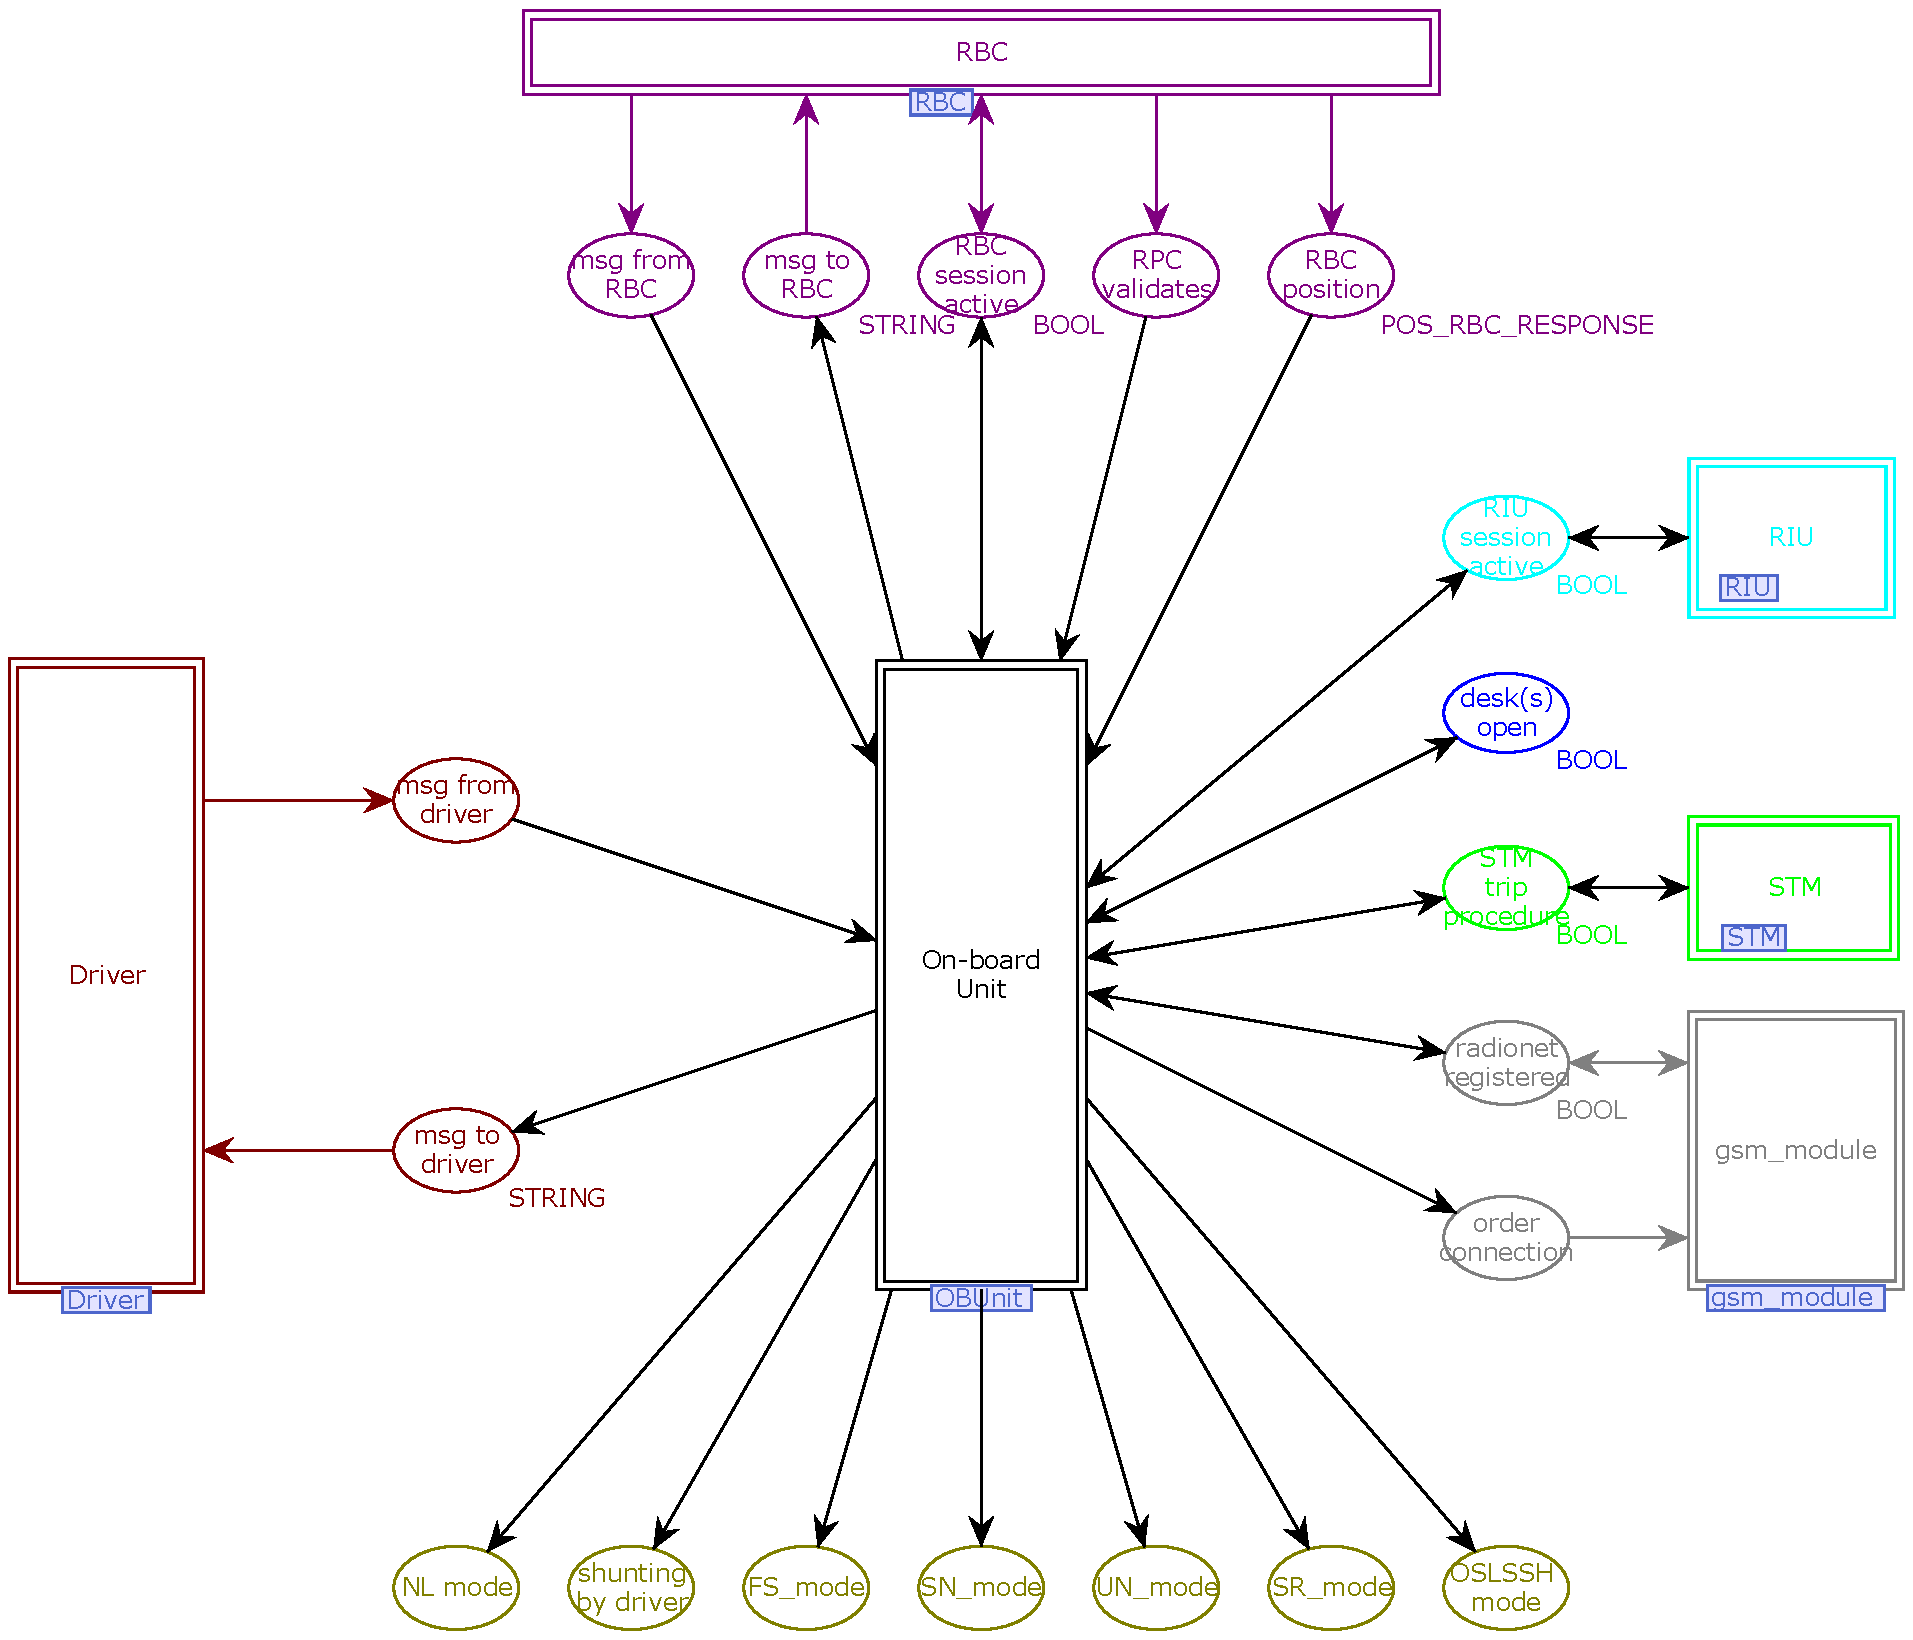
\includegraphics[width=0.9\textwidth]{figures/Top.pdf}
	\caption{Top level model}
	\label{fig:Top}
\end{figure}

Zooming in subpage \texttt{On-board Unit} yields the CPN model in Fig.~\ref{fig:OBUnit}. This CPN model has two subpages: Subpage \texttt{Start} models the states S0 and S1 of the specification (i.e., Subset-026 chapter 5.4) and subpage \texttt{Rest} the remaining states. At this level of abstraction, we see on the left hand side seven places (green frame). Each such place models (a part) of the state of the on-board unit, for example, the mode and the train running number. The current model has 689 places, 173 transitions and 1,227 arcs.

\begin{figure}[tb]
	\centering
		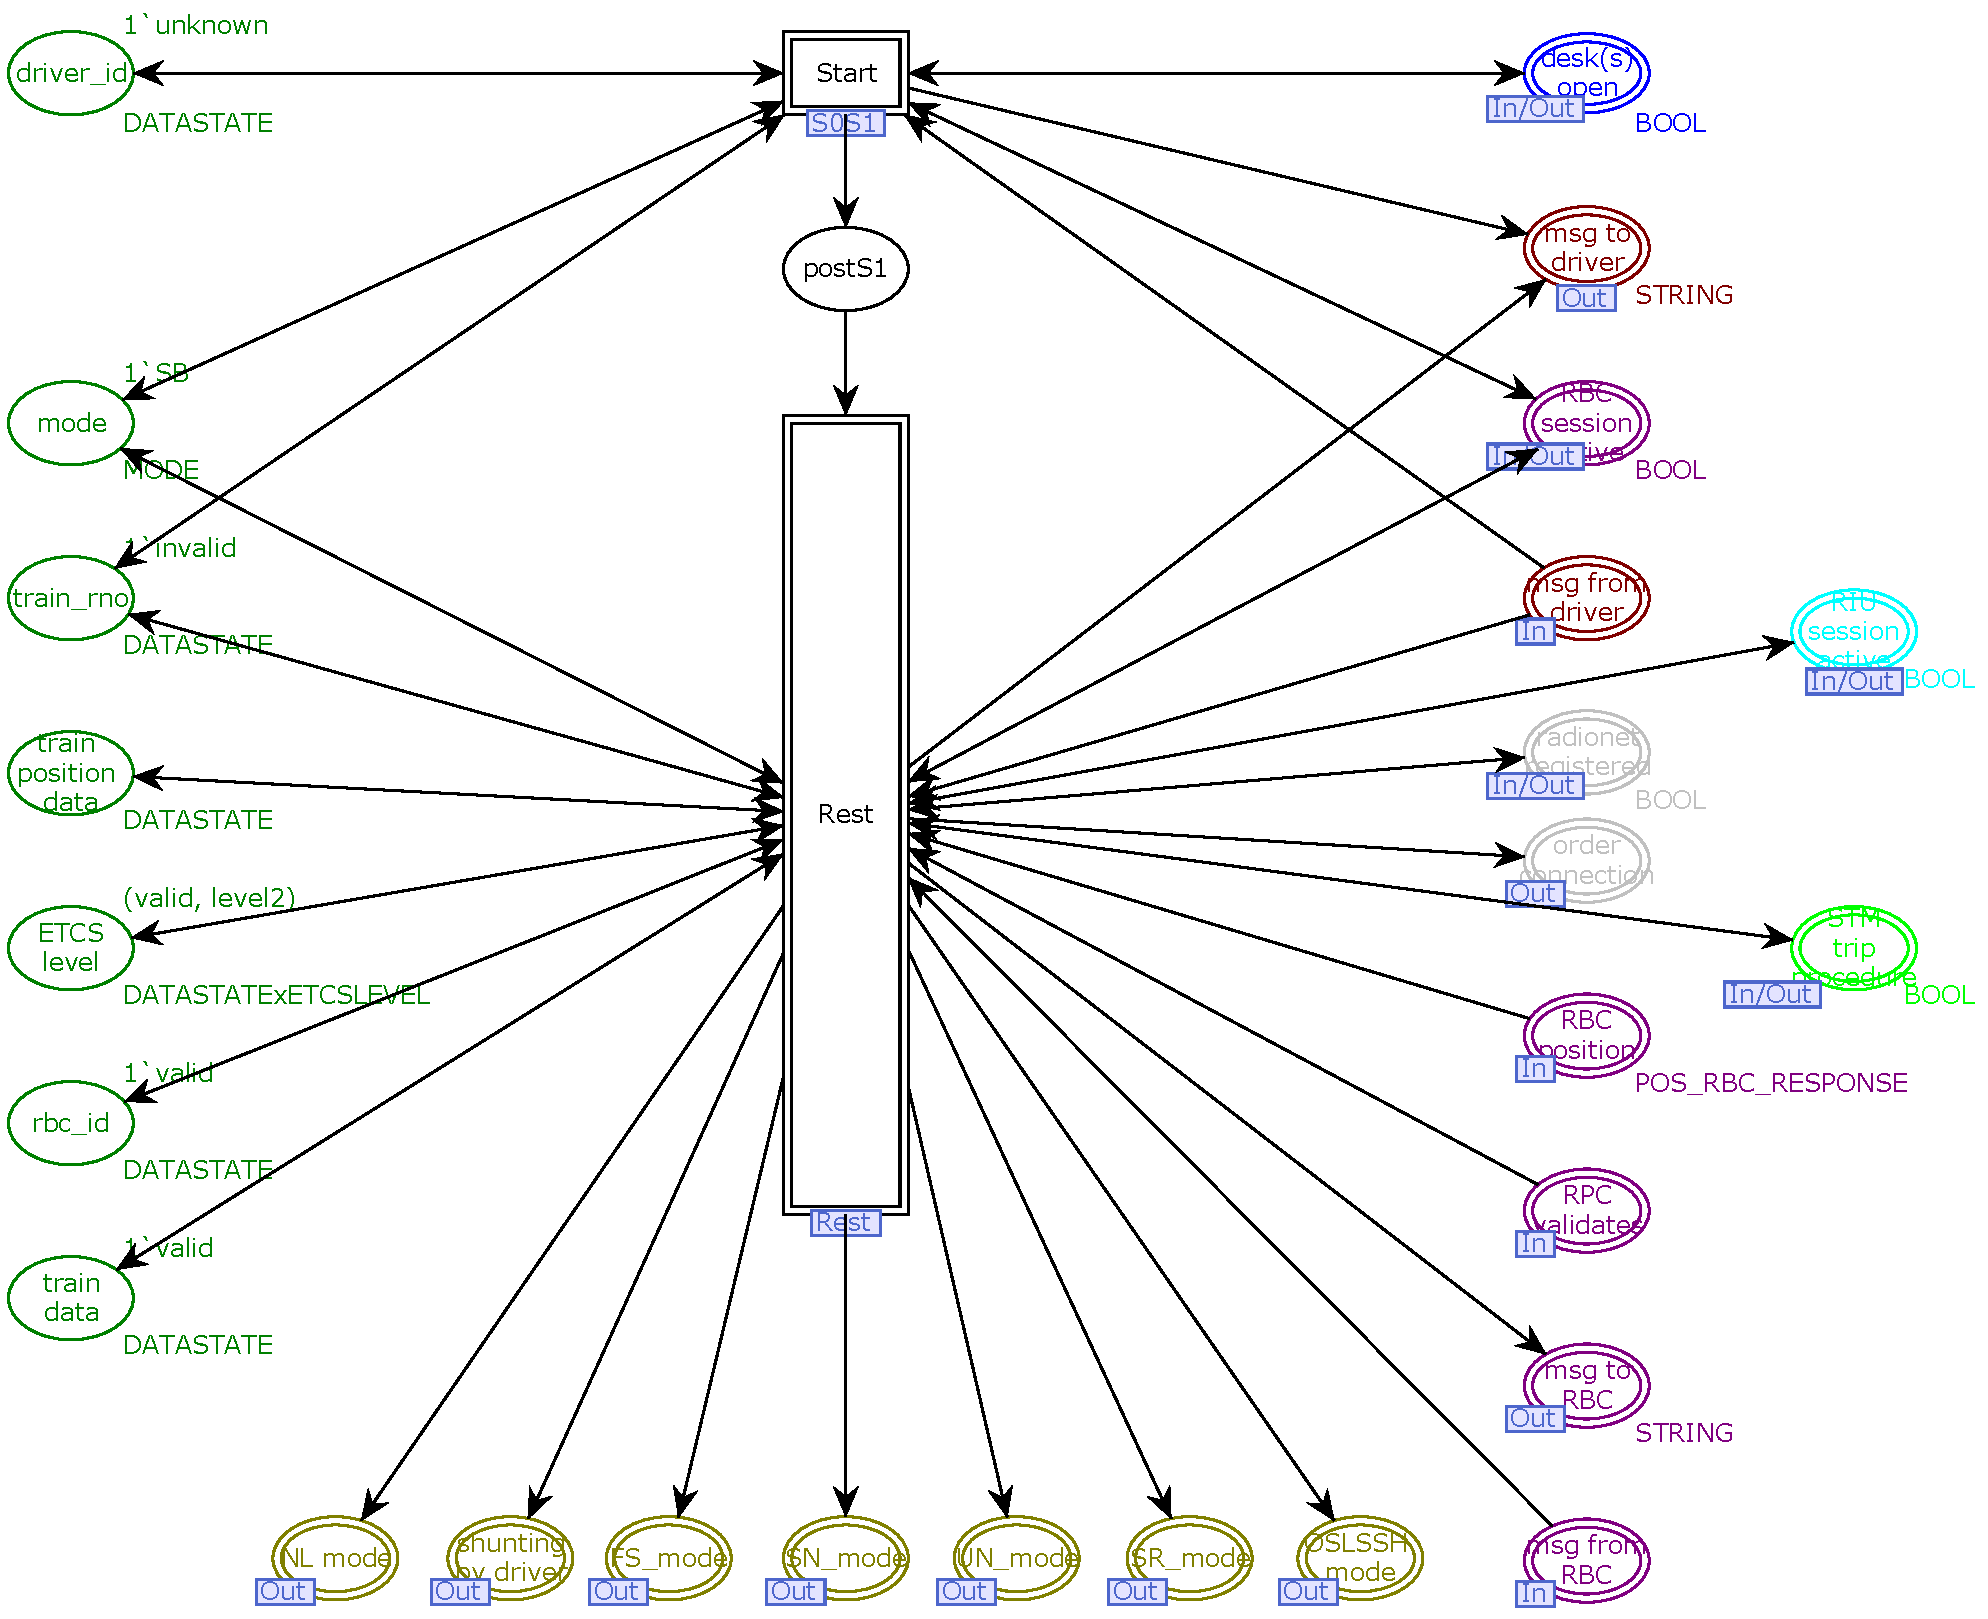
\includegraphics[width=0.9\textwidth]{figures/OBUnit.pdf}
	\caption{CPN model of the on-board unit}
	\label{fig:OBUnit}
\end{figure}

Having a more detailed look at Fig.~\ref{fig:OBUnit}, we observe that our model does not represent all variables of the on-board unit as given in the specification and also partially abstracts from data. We abstract from those details, because the model is tailored to formalize the \textit{control flow} of the on-board unit and, in particular, the \textit{communication behavior} with its environment. As a benefit, this abstraction reduces the complexity of the model and improves its understandability. Additional details, such as data and precise message values, can be added in a refinement step.

The modeled procedures have been manually modeled using CPN Tools. Thereby, each element in the model has been reviewed against the respective requirement, as given in the specification. To improve the confidence in the model, in a second step, a person other than the modeler checked the model against the specification. In addition, we used the simulator to check whether the modeled behavior of the CPN matched the intended behavior.

So far, the primary goal of modeling has been to validate the specification. During the modeling we discovered 36 inconsistencies, ambiguities and gaps in the specification which we reported in~\cite{specfindings}. 


\subsection{Means}

The input for our approach is the specification described in Subset-026 chapter 5. Our output is a CPN model and a report describing inconsistencies, ambiguities and gaps in the Subset-026 chapter 5.


\section{Results}

\subsection{Summary}

We have modeled the following five procedures of Subset-026 chapter 5 as CPN:
\begin{itemize}
	\item Start of Mission (Subset-026 chapter 5.4)
	\item End of Mission (Subset-026 chapter 5.5)
	\item Shunting Initiated by Driver (Subset-026 chapter 5.6)
	\item Override (Subset-026 chapter 5.8)
	\item Train Trip (Subset-026 chapter 5.11)
\end{itemize}

%During the modeling we discovered 36 inconsistencies, ambiguities and gaps in the %specification which we reported in~\cite{specfindings}. 
Our CPN models the system behavior---that is, the interplay between the different entities of the ETCS---and partially abstract from data. Therefore, we complement the work on SysML modeling, where the focus is on the connectivity of components and the data types.
 
\subsection{Conclusions/Lessons learned}
 
The numerous specification findings illustrate the need for validating the specification. CPNs are well-suited to model the behavioral aspects described in Subset-026 chapter 5. The size of the model clearly indicates the complexity of the procedures, even at the current level of abstraction. Therefore, we expect that applying formal verification on the resulting CPNs will not be feasible due to state-space explosion.

\section{Future Activities}


We shall continue our work by completing the model, contributing to the modeling of (parts of) Subset-026 chapter 5 using SCADE, and verifying the SCADE model. In addition, we are planning to exploit synergies by collaborating with the project partner LAAS who advocate the Petri net model checker TINA~\cite{BerthomieuV2006}. In addition, we are working with the project partners from Braunschweig University of Technology on generating test cases from the CPN model.


\section{Modeling the Subset-026 chapter 5}

We plan to model the remaining parts of Subset-026 chapter 5, thereby reporting possible additional findings in the specification. The goal is to have a CPN modeling all procedures that are described in Subset-026 chapter 5. We also want to compare our model with the (corresponding part of the) ERTMSFormalSpec model~\cite{ertms}.


\section{SCADE Modeling}

As the ETCS will be modeled using SCADE, we shall contribute to this modeling process. To use the experience that we gained from modeling Subset-026 chapter 05 with CPN Tools, we want to contribute to the SCADE modeling of (parts of) the Subset-026 chapter 5. The SCADE design flow starts with modeling all components and their interplay using SysML block diagrams (with the tool SCADE Designer). The resulting SysML diagrams provide a functional and an architectural view. They are similar to the CPN model in Fig.~\ref{fig:Top}. In a second step, the behavior of each block has to be fully modeled on the system level using SCADE Suite. Currently, SCADE does not support state machine models on the level of SysML. Our CPN model provides this level of abstraction and will, therefore, be useful for the SCADE modeling.


\subsection{Verification of the SCADE Model}

Another task concerns the verification of the resulting SCADE model. Recently, researchers reported on complexity problems already for medium-sized SCADE models that restrict the verification using the SCADE prover~\cite{HuhnM2014scp,DaskayaHM2011fmics}. Given the complexity of the ETCS, we assume that we will face similar challenges. To alleviate those complexity problems, we aim to apply the following three techniques:

\begin{description}
	\item[Abstraction:] We will apply abstraction techniques on the SCADE model to prove safety properties on a higher level of abstraction whenever possible. On the one hand, we can apply SCADE contracts to restrict the domain of the input values. This technique is known as environment abstraction. On the other hand, we can transform the SCADE model into a model of higher abstraction, thereby using different formalisms such as timed automata, transition systems and Petri nets. (As SCADE has a formal semantics such transformations are possible, but may take considerable effort.) We can then use verification tools that are dedicated to the properties of interest and the chosen formalism. We see the chance that our CPN model can be used for this task, too. For example, Uppaal~\cite{BehrmannDLHPYH2006} can analyze timed automata, the Spin model checker~\cite{Holzmann97} and NuSMV~\cite{CimattiCGGPRST2002} can analyze transition systems, and TINA~\cite{BerthomieuV2006}, LoLA~\cite{Wolf2007}, and CPN Tools~\cite{Westergaard2013apn} are tools for analyzing (different variants of) Petri nets.
	%
	\item[Compositional Reasoning:] Another approach is to prove properties for individual components and deduce from it the correctness of a property concerning the entire ETCS. Here we think that we can, in particular, combine our model with the MoRC model~\cite{braunstein_MorC_2013} and apply compositional reasoning.
	%
	\item[Correctness by Design:] The two previous approaches support \textit{correctness by verification}; that is, first the model is designed and in the next step it is verified. A different methodology is \textit{correctness by design}. The idea is to model on a higher level of abstraction and to prove that certain safety properties hold. Then the model is iteratively refined. Each refinement step has to guarantee that all properties that hold for the more abstract level also hold in the refined model. The challenge is to find property-preserving refinement rules or a refinement relation between an abstract model and a refined model that preserves the desired properties and to verify that this relation holds. The results can be applied to validate the SCADE model and the specification.
\end{description}



